\documentclass[aspectratio=169,11pt,hyperref={colorlinks=true}]{beamer}
\usetheme{boxes}
\setbeamertemplate{navigation symbols}{}
\definecolor{IBMblue}{RGB}{31,112,193}
\setbeamercolor{titlelike}{fg=IBMblue}
\setbeamercolor{structure}{fg=IBMblue}
\hypersetup{colorlinks,urlcolor=IBMblue}
\setbeamertemplate{footline}[frame number]
% Inserting graphics
\usepackage{graphicx}
% Side-by-side figures, etc
\usepackage{subfigure}
% Code snippits
\usepackage{listings}
\usepackage{minted}

\usepackage{lmodern}
% Color stuff
\usepackage{color}
\usepackage{amsmath}
\usepackage{tikz}
\usepackage{gensymb}
\newcommand\RBox[1]{%
  \tikz\node[draw,rounded corners,align=center,] {#1};%
}
\usepackage{hyperref}
%\usecolortheme{buzz}
%\usecolortheme{wolverine}
%\usetheme{Boadilla}
\usepackage[T1]{fontenc}

\definecolor{mygreen}{rgb}{0,0.6,0}
\definecolor{mygray}{rgb}{0.5,0.5,0.5}
\definecolor{mymauve}{rgb}{0.58,0,0.82}

\lstset{%
  backgroundcolor=\color{white},   % choose the background color; you must add \usepackage{color} or \usepackage{xcolor}
  breakatwhitespace=false,         % sets if automatic breaks should only happen at whitespace
  breaklines=true,                 % sets automatic line breaking
  captionpos=b,                    % sets the caption-position to bottom
  commentstyle=\color{IBMblue},  % comment style
  extendedchars=true,              % lets you use non-ASCII characters; for 8-bits encodings only, does not work with UTF-8
  keepspaces=true,                 % keeps spaces in text, useful for keeping indentation of code (possibly needs columns=flexible)
  keywordstyle=\color{blue},       % keyword style
%  otherkeywords={*,...},           % if you want to add more keywords to the set
  numbersep=5pt,                   % how far the line-numbers are from the code
  numberstyle=\tiny\color{mygray}, % the style that is used for the line-numbers
  rulecolor=\color{black},         % if not set, the frame-color may be changed on line-breaks within not-black text (e.g. comments (green here))
  showspaces=false,                % show spaces everywhere adding particular underscores; it overrides 'showstringspaces'
  showstringspaces=false,          % underline spaces within strings only
  showtabs=false,                  % show tabs within strings adding particular underscores
  stringstyle=\color{IBMblue},   % string literal style
}


\setbeamerfont{caption}{series=\normalfont,size=\fontsize{6}{8}}
\setbeamertemplate{caption}{\raggedright\insertcaption\par}

\setlength{\abovecaptionskip}{0pt}
\setlength{\floatsep}{0pt}

\author[Matthew Treinish]{%
    \texorpdfstring{%
        \centering
        Matthew Treinish\\
        Developer Advocate - IBM \\
        \href{mailto:mtreinish@kortar.org}{mtreinish@kortar.org}\\
        \texttt{mtreinish on Freenode}\\
        \href{https://github.com/mtreinish/intro-to-docker}{https://github.com/mtreinish/intro-to-docker}
   }
   {Matthew Treinish}
}
\date{July 9th, 2018}

\title{Introduction to Docker}
\begin{document}

\titlepage

\section{What is Docker?}
\begin{frame}
    \frametitle{What is Docker?}
    \begin{columns}[T]
        \begin{column}{.48\textwidth}
            \begin{itemize}
                \item Tooling to manage platform
                \item Manages the lifecycle of containers
                \item Simplified existing technologies for ease of use
            \end{itemize}
        \end{column}
        \begin{column}{.48\textwidth}
            
\includegraphics[width=.9\textwidth]{Docker_logo.png}
        \end{column} 
    \end{columns}
\end{frame}

\begin{frame}
    \frametitle{Containers}
    \begin{itemize}
    \item A group of processes run in isolation
        \begin{itemize}
            \item Similar to VMs by managed at the process level
            \item Run on a shared kernel
        \end{itemize}
    \item Each container has its own namespaces
        \begin{itemize}
            \item \textbf{PID} process IDs
            \item \textbf{USER} user and group IDs
            \item \textbf{LTS} hostname and domain name
            \item \textbf{NS} mount points
            \item \textbf{NET} network devices, stacks, ports
            \item \textbf{IPC} inter-process communications, message queues
            \item \textbf{cgroups} controls limits and monitoring of resources
        \end{itemize}
    \end{itemize}
\end{frame}

\begin{frame}
    \frametitle{Containers vs VMs}
    \centering
    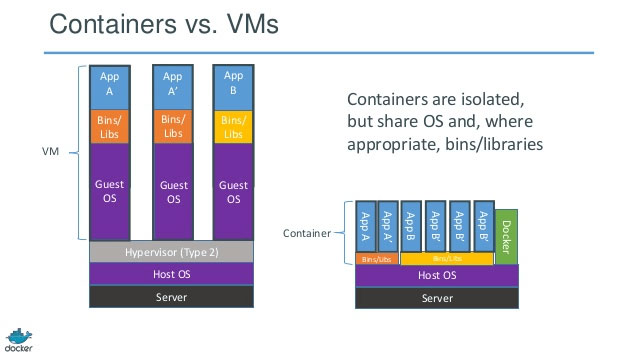
\includegraphics[width=.9\textwidth]{containers-vs-vm.jpg}

\end{frame}

\section{Getting Started with Docker}
\subsection{Interacting with Docker}
\begin{frame}
    \frametitle{First container}
    \textbf{\$ docker run ubuntu echo Hello World} \\
\end{frame}

\begin{frame}
    \frametitle{What Happened}
    \begin{itemize}
        \item Docker created a directory with a ubuntu filesystem (image)
        \item Docker created a new set of namespaces
        \item Ran a new process: echo Hello World
        \item Using those namespaces to isolate it from other processes
        \item Using that new directory as the root of the filesystem (chroot)
        \item That's it!
        \item Notice as a user I never installed ubuntu
        \item Run it again, notice how quickly it ran
    \end{itemize}
\end{frame}

\begin{frame}
    \frametitle{ssh-ing into a container}
    \textbf{\$ docker run -ti ubuntu bash}
    \begin{itemize}
        \item Now the process is \textit{bash} instead of \textit{echo}
        \item But its still just a process
        \item Look around, mess around, its isolated
    \end{itemize}
\end{frame}

\begin{frame}
    \frametitle{Look under the covers}
    \textbf{\$ docker run ubuntu ps -ef} \\
    \\
    Things to notice with these examples:
    \begin{itemize}
        \item Each container only sees its own processes
        \item Running as root
        \item Running as PID 1
    \end{itemize}

\end{frame}
\subsection{Docker Images}
\begin{frame}
    \frametitle{Docker images}
        
\end{frame}

\begin{frame}
    \frametitle{Layering}
    \begin{itemize}
        \item Docker uses a copy-on-write (union) filesystem
        \item New files (or modifications) are only visible to current/above layers
        \item Layers allow for reuse
        \item Images are tarballs of layers
    \end{itemize}
\end{frame}

\begin{frame}
    \frametitle{Dockerhub}
    \href{https:/hub.docker.com}{https://hub.docker.com}
    \begin{itemize}
        \item Public registry of Docker Images
        \item Hosted by Docker Inc.
        \item Free for public images
        \item By default docker engines will look in DockerHub for images
        \item Browser interface for searching, descriptions of images
    \end{itemize}
\end{frame}

\section{Building Images}
\begin{frame}
    \frametitle{The Dockerfile}
    
\end{frame}

\section{Image Registry}
\begin{frame}
    \frametitle{DockerHub}

\end{frame}



\section{Questions?}
\begin{frame}
\frametitle{Where to get more information}

\end{frame}

\end{document}
